\documentclass[tikz,border=5pt]{standalone}


\usetikzlibrary{calc}


\begin{document}
    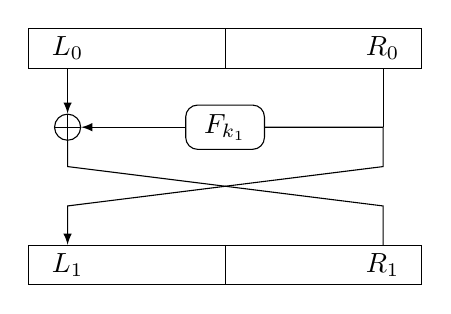
\begin{tikzpicture}
        % 1. Function F_k1 and XOR Node
        \node (f1) at (0,-1.5cm) [minimum width=1cm,rounded corners=1ex,draw] {$F_{k_1}$};
        \node (xor1) [left of = f1, circle, node distance = 2cm, draw] {};
        \draw[-] (xor1.north) -- (xor1.south);
        \draw[-] (xor1.east) -- (xor1.west);
        \draw[-latex] (f1.west) -- (xor1.east);

        % 2. Top Block (L0, R0)
        \node (p0) [above of = f1, minimum width=5cm,minimum height=0.5cm,node distance=1cm,draw] {};
        \node (l0) [above of = xor1,node distance=1cm] {$L_0$};
        \node (r0) [right of = l0, node distance = 4cm] {$R_0$};
        \draw[-] (p0.north) -- (p0.south);
        
        % Connections from Top Block
        \draw[-latex] (l0 |- p0.south) -- (xor1.north); 
        \draw[-] ($(f1.east)+(1.5cm,0)$) -- +(0,0.75cm); 

        % 3. Bottom Block (L1, R1)
        \node (p1) [below of = f1, minimum width=5cm,minimum height=0.5cm,node distance=1.75cm,draw] {}; 
        \node (l1) [below of = xor1,node distance=1.75cm] {$L_1$};
        \node (r1) [right of = l1, node distance = 4cm] {$R_1$};
        \draw[-] (p1.north) -- (p1.south);
        
        % 4. Cross-wiring 
        % Right side to Left side (R0 -> L1)
        \draw[-latex] (f1.east) -| +(1.5cm,-0.5cm) -- ($(xor1) - (0,1cm)$) -- (xor1 |- p1.north);
        
        % Left side to Right side (L0/XOR -> R1)
        \draw[-] (xor1.south) -- ($(xor1)+(0,-0.5cm)$) -- ($(f1.east) + (1.5cm,-1cm)$) -- +(0,-0.5cm);
        
    \end{tikzpicture}
\end{document}